% Segment of a Cylinder
% Author: Mathias Magdowski
\documentclass[tikz,border=10pt]{standalone}
\usepackage{tikz}
\usetikzlibrary{calc}

\begin{document}
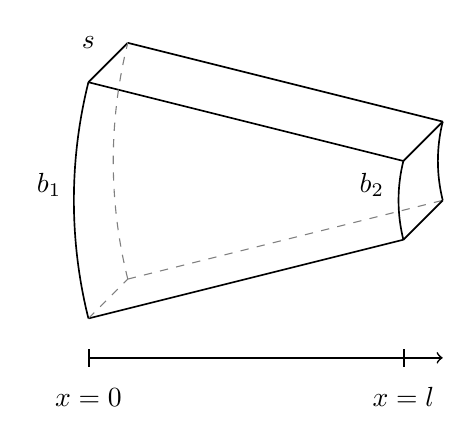
\begin{tikzpicture}
	% general shift to north east
	\coordinate (O) at (0.5,0.5);
	\draw[semithick] (0,0) -- (4,1);% bottom line in front
	\draw[dashed,color=gray] (O) -- ($(4,1)+(O)$);% bottom line in the back
	\draw[semithick] (0,3) -- (4,2);% top line in front
	\draw[semithick] ($(0,3)+(O)$) -- ($(4,2)+(O)$);% top line in the back
	\draw[semithick] (0,3) -- ($(0,3)+(O)$);% line to the back, top left
	\draw[semithick] (4,2) -- ($(4,2)+(O)$);% line to the back, top right
	\draw[semithick] (4,1) -- ($(4,1)+(O)$);% line to the back, bottom right
	\draw[dashed,color=gray] (0,0) -- (O);% line to the back, bottom left
	% the first angle is 180°+atan(0.25)
	% the second angle is 180°-atan(0.25)
	% the radius is sqrt(6^2+1.5^2)
	\draw[semithick] (0,0) arc (194.036:165.964:6.185);% left arc in front
	\draw[dashed,color=gray] (O) arc (194.036:165.964:6.185);% left arc in the back
	% the first angle is 180°+atan(0.25)
	% the second angle is 180°-atan(0.25)
	% the radius is 1/3*sqrt(6^2+1.5^2)
	\draw[semithick] (4,1) arc (194.036:165.964:2.062);% right arc in front
	\draw[semithick] ($(4,1)+(O)$) arc (194.036:165.964:2.062);% right arc in the back
	\draw (-0.5,1.7) node {$b_1$};
	\draw (3.6,1.7) node {$b_2$};
	\draw (0,3.5) node {$s$};
	\draw[|-,semithick] (0,-0.5) -- (4,-0.5);
	\draw[|->,semithick] (4,-0.5) -- (4.5,-0.5);
	\draw (0,-1) node {$x=0$};
	\draw (4,-1) node {$x=l$};
\end{tikzpicture}
\end{document}